Let $(\R^{1 + 2}, m)$ be the $(1 + 2)$-dimensional Minkowski space-time, and suppose $(\cM, g)$ is a compact Riemannian manifold. By Nash's theorem, we can view the target manifold extrinsically via an isometric embedding $\cM \hookrightarrow \R^N$, denoting the second fundamental form by $\II : T\cM \times T\cM \to T \cM^\perp$. We say that $\phi : \R^{1 + 2} \to \cM$ solves the \emph{wave maps equation} if 
\begin{equation}
	\begin{split}
		\Box \phi^a 
			&= - \II^a_{bc} (\phi)  \partial^\alpha \phi^b \partial_\alpha \phi^c, \\
		\phi_{|t = 0}
			&= \phi_0 ,\\
		\partial_t \phi_{|t = 0}
			&= \phi_1,	
	\end{split}
	\label{eq:wave}
	\tag{WM}
\end{equation}
for initial data $(\phi_0, \phi_1)$ satisfying the constraints $\phi_0 (x) \in \cM$ and $\phi_1 (x) \in T_{\phi_0 (x)} \cM$. 

\subsection{Conservation laws}

Formally, wave maps are critical points of the Lagrangian
	\[ \cL [\phi] := \int_{\R^{1 + 2}} \langle\partial^\alpha \phi, \partial_\alpha \phi \rangle_g \, dt dx \]
of which the wave maps equation \eqref{wave} is the Euler-Lagrange equation. There is a corresponding stress-energy tensor 
	\[ 
		T_{\alpha\beta} [\phi] := \langle \partial_\alpha \phi, \partial_\beta \phi \rangle_g  - \frac12 m_{\alpha \beta} \langle \partial^\gamma \phi, \partial_\gamma \phi \rangle_g
	 \]
which is divergence-free
	\[ \partial^\alpha T_{\alpha \beta} [\phi] = 0. \]
Then, contracting the stress-energy tensor with the vector field $\partial_t$, applying the divergence-free condition and Stokes' theorem on the space-time slab $I \times \R^2$ furnishes conservation of the \emph{Dirichlet energy} for solutions to the wave maps equation, 
	\[ \cE[\phi (t)] := ||\vec \phi||_{\dot H^1 \times L^2}^2 (t) = \int_{\R^2} |\partial_t \phi|^2 + |\nabla_x \phi|^2 \, dx , \]
where we have denoted $\vec \phi (t) = (\phi, \partial_t \phi) (t)$. In view of Noether's theorem, conservation of energy corresponds to the time-translation symmetry of the Lagrangian $\cL [\phi]$. Note that the wave maps equation and its Lagrangian are invariant with respect to the scaling 
	\[ \phi(t, x) \mapsto \phi(\lambda t, \lambda x). \]
The Dirichlet energy is also invariant with respect to this scaling in $(1 + 2)$-dimensions and coincides precisely with the \emph{energy space} $\vec \phi (t) \in \dot H^1_x \times L^2_x$, thus, we refer to the wave maps equation \eqref{wave} on $\R^{1 + 2}$ as \emph{energy-critical}. 	

If we instead integrated the stress-energy tensor over the light cone, we can obtain a monotonicity formula for the energy when restricted to slices of the light cone in time. Before we state the formula, we will need to introduce some notation. We denote the forward light cone by 
	\[ C := \{(t,x ) \in \R^{1 + 2} : r \leq t\} \]
and its restrictions to some time interval $I \subseteq [0, \infty)$ as well as time-slices by 
	\begin{align*}
		C_I 
			&:= C \cap (I \times \R^2), \\
		S_{t}
			&:= C \cap (\{t\} \times \R^2).
	\end{align*}
The \emph{null boundary} $\partial C_I$ denotes the boundary of the time-slab $C_I$ modulo the top and bottom time-slices. Due to singularities on the null boundary, we will also consider the shifted light cone 
	\[ C^\delta := (\delta, 0) + C. \]
Accordingly, we have 
	\begin{align*}
		C^\delta_I
			&:= C_I \cap C^\delta, \\
		S^\delta_t
			&:= S_t \cap C^\delta,		
	\end{align*}	
In view of the null boundary, we define the null frame $\{L, \underline L, \slashed\partial\}$ to be the vector fields given by 
	\begin{align*}
		L
			&:= \partial_t + \partial_r, \\
		\underline L
			&:= \partial_t - \partial_r,\\
		\slashed \partial
			&:= \frac1r \partial_r . 		
	\end{align*}
	
	
	\begin{figure}[h]
		\begin{center}
			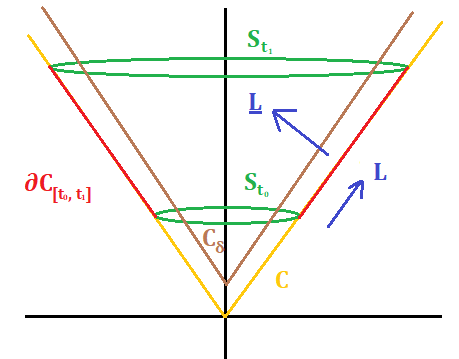
\includegraphics{graphics/cone}
			\caption{The light cone $C$, its vertical shift $C^\delta$, the time-slices $S_{t}$, the null boundary $\partial C_{[t_0, t_1]}$, and the null frame $\{L, \underline L, \slashed\partial\}$. }
		\end{center}	
	\end{figure}	
Contracting the stress-energy tensor $T_{\alpha \beta}$ with the vector field $\partial_t$ and then integrating then over the slab of the light cone $C_{[t_0, t_1]}$, we obtain in view of the divergence-free property and Stokes' theorem the  \emph{monotonicity formula}
	\begin{equation}
		\cE_{S_{t_1}} [\phi] = \cF_{[t_0, t_1]} [\phi] + \cE_{S_{t_0}} [\phi],
		\label{eq:mono}
		\tag{$\uparrow$}
	\end{equation}	
where $\cE_{S_{t_0}} [\phi]$ denotes the energy on the time-slice $S_{t_0}$, 
	\[ \cE_{S_{t_0}} [\phi] := \int_{S_{t_0}} |\partial_t \phi|^2 + |\nabla_x \phi|^2 \, dx ,\]
and $\cF_{[t_0, t_1]} [\phi]$ denotes the \emph{flux} of the wave map on the null-boundary of the light cone,
	\[
		\cF_{[t_0, t_1]} [\phi] := \int_{\partial C_{[t_0, t_1]}} \left( \frac14 |L \phi|^2 + \frac12 |r^{-1} \partial_\theta \phi|^2 \right) \, dA.
	\]
The key observation is that the flux is non-negative, hence \eqref{mono} is indeed a monotonicity formula for the energy on time-slices of the light cone $\cE_{S_t} [\phi] \nearrow$. In particular, we can define the energy at the tip of the light cone and at infinity by 
	\begin{align*}		
		\cE_0 
			&:= \lim_{t \searrow 0} \cE_{S_t} [\phi], \\
		\cE_\infty 
			&:= \lim_{t \nearrow \infty} \cE_{S_t} [\phi]. 
	\end{align*}


\subsection{Main results}

We consider the initial data problem for the wave maps equations \eqref{wave} on $\R^{1 + 2}$ with finite energy data $\vec \phi_0 \in \dot H^1_x \times L^2_x$. Global well-posedness where the target manifold is a sphere $\cM = \mathbb S^k$ was established in \cite{Tao2001} and for general targets in \cite{Tataru2005}. In this note we turn towards addressing the following questions for large initial data:
	\begin{itemize}
		\item global well-posedness, 
		\item scattering.
	\end{itemize}
We restrict our attention to the forward light cone. For blow-up, we use time-reversibility of the equation and finite speed of propagation. For scattering, we choose a ball $B$ large so that energy is small outside of this ball, so the small data theory applies. Hence it remains to study the influence cone of $B$. 


\begin{theorem}[Bubbling theorem]
	Let $\phi$ be a wave map which is singular at $(0, 0)$, respectively $\phi \not\in \cS [t_\infty, \infty)$, then there exists a sequence $\lambda^0_\nu \searrow 0$, respectively $(\lambda^\infty_\nu \nearrow \infty)$ such that rescaling 
		\[ \phi_\nu (t, x) := \phi(\lambda^0_\nu t, \lambda^0_\nu x), \qquad \text{respectively }  \phi_\nu (t, x) := \phi(\lambda^\infty_\nu t, \lambda^\infty_\nu x),\]
	we can find a sequence of concentration points $(t_\nu, x_\nu) \in C^{1/2}_{[1, O(1)]}$ and scales $r_\nu \searrow 0$ for which
		\[ \phi_\nu (t_\nu + r_\nu t, x_\nu + r_\nu x) \to \omega (t, x) \]
	for some non-constant soliton $\omega$. 
\end{theorem}

\begin{theorem}[Threshold theorem]
	The wave maps equation is globally well-posed for all initial data below the energy threshold and the corresponding solutions scatter in the following sense:
	\begin{enumerate}
		\item (regular data) For regular data $\vec \phi_0$, then there exists a unique global regular solution which has Lipschitz dependence on the initial data locally in time in the $\dot H^1 \times L^2$ topology. 
		
		\item (rough data) The flow map admits an extension to rough data. 
		
		\item (weak Lipschitz dependence) The flow map is globally Lipschitz in the $\dot H^{\sigma}$ topology for $\sigma < 1$ close to $1$. 
		
		\item (scattering) The $\cS^1$ norm is finite.
	\end{enumerate}	
\end{theorem}

\begin{theorem}[Dichotomy theorem]
	The wave maps equation \eqref{wave} is locally well-posed for arbitrary finite energy data. Further, one of the following two properties must hold for the forward maximal solution:
	\begin{enumerate}
		\item the solution is global, scatters at infinity,
		\item bubbling off a soliton. 
	\end{enumerate}
\end{theorem}

